\chapter{Grundlagen}

\section{Mathematische Grundlagen}

Diese Sektion beschreibt die wesentlichen mathematischen Konzepte, die in dieser Arbeit zur Verwendung kommen.

\subsection{Konventionen}

Transformationen werden im Folgenden folgendermaßen betitelt: \improvement{Konventionen einfügen}

\subsubsection{Karte}

Die Bezeichnung (TSDF-)Karte beziehungsweise \textbf{Map} wird im Folgenden für die implizite TSDF Repräsentation der Umgebung verwendet.
Sie bezeichnet zusätzlich das Weltkoordinatensystem.

\subsubsection{Pfad}

\improvement{Schreiben über Pfad (indizierung, grobe Mathe), Posen, relative und absolute Transformationen}

\subsection{Koordinatensysteme}

Ein wesentliches Konzept bei der Verarbeitung räumlicher Daten ist die Verwendung von Koordinatensystemen.
Sie werden genutzt um die Positionen von Daten und Objekten im Raum zu beschreiben.
Koordinatensysteme können für sich alleine stehen oder relativ zu anderen Koordinatensystemen.
Im Dreidimensionalen besitzt ein Koordinatensystem drei verschiedene Achsen (x, y und z-Achse), die jeweils im 90 Grad Winkel zueinander ausgerichtet sind.
Rotationen im Raum werden beschrieben als Rotationen um die jeweiligen Achsen.
Welche Achse in welche Richtung zeigt ist nicht eindeutig definiert.
Es gibt jedoch verschiedene Standards beziehungsweise Konventionen wie das links- oder rechtshändische Koordinatensystem.
In ROS wird konventionell ein rechtshändisches Koordinatensystem, abgebildet in Abbildung \ref{fig:ros_coordinate_sys} dargestellt. Dies wird im Folgenden ebenfalls als Standard verwendet.

\begin{figure}
		\centering
		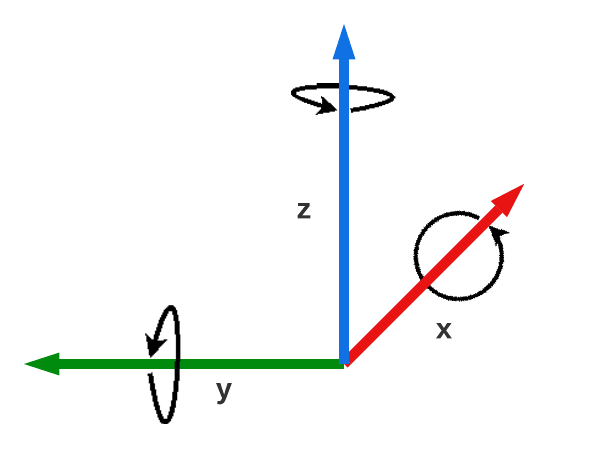
\includegraphics
			[scale=0.35]
			{ros_coordinate_sys}
		\caption
			[Caption for LOF]{Schematische Darstellung der Konvention für Koordinatensysteme im ROS Framework. Die z-Achse zeigt nach oben, die x-Achse nach vorne und die y-Achse nach links. Die Rotation um die Achsen ist entsprechend der Konvention im Uhrzeigersinn.}			                                                                                                                                     
		\label{fig:ros_coordinate_sys}
	\end{figure}

In der Robotik kommt es häufig vor, dass verschiedene (bewegliche) Komponenten relativ zu einem globalen Bezugssystem oder relativ zueinander beschrieben werden müssen. Die Bewegung eines übergeordneten Bezugssystems kann implizit für eine Veränderung der relativ zu diesem Bezugssystem platzierten Systeme führen.
Dies lässt sich anhand eines Arm-Roboters zeigen, der mehrere miteinander verbundene Gelenke hat. Bewegt sich ein Gelenk werden automatisch auch die am Arm weiter außen befindlichen Gelenke mitbewegt. Aus Sicht des bewegten, übergordneten Bezugssystems hat sich die Position der untergeordneten Gelenke nicht verändert, aus Sicht des globalen Bezugssystems, wie zum Beispiel dem Montierungspunkt des Roboters, allerdings schon.

In ROS werden Anhängigkeiten zwischen Bezugssystemen in einer Baumstruktur, genannt \textit{transformation tree (tf-tree)} dargestellt.
Die Wurzel dieser Baumstruktur ist das globale Bezugssystem, wie zum Beispiel der Ursprung einer globalen Karte oder der Startpunkt der Trajektorie eines Roboters.
Das globale Bezugssystem kann beliebig gewählt werden.
Auf diese Weise kann ein Koordinatensystem, welches relativ zu einem anderen gelegen ist im Baum als Kindknoten seinem Bezugssystem untergeordnet werden. Es wird nur die relative Transformation (s. Kapitel \ref{section:transformationen}) zwischen den Systemen im Baum gespeichert.
Dies hat den Vorteil, dass bei der Bewegung eines Systems die untergordneten Systeme nicht ebenfalls verändert werden müssen, da deren Transformationen relativ zum bewegten Bezugssystem angegeben sind und nicht global zur Wurzel des Baumes.
Abbildung \ref{fig:robot_tf} zeigt ein Beispiel für einen Roboter mit mehreren voneinander abhängigen System.


\begin{figure}
		\centering
		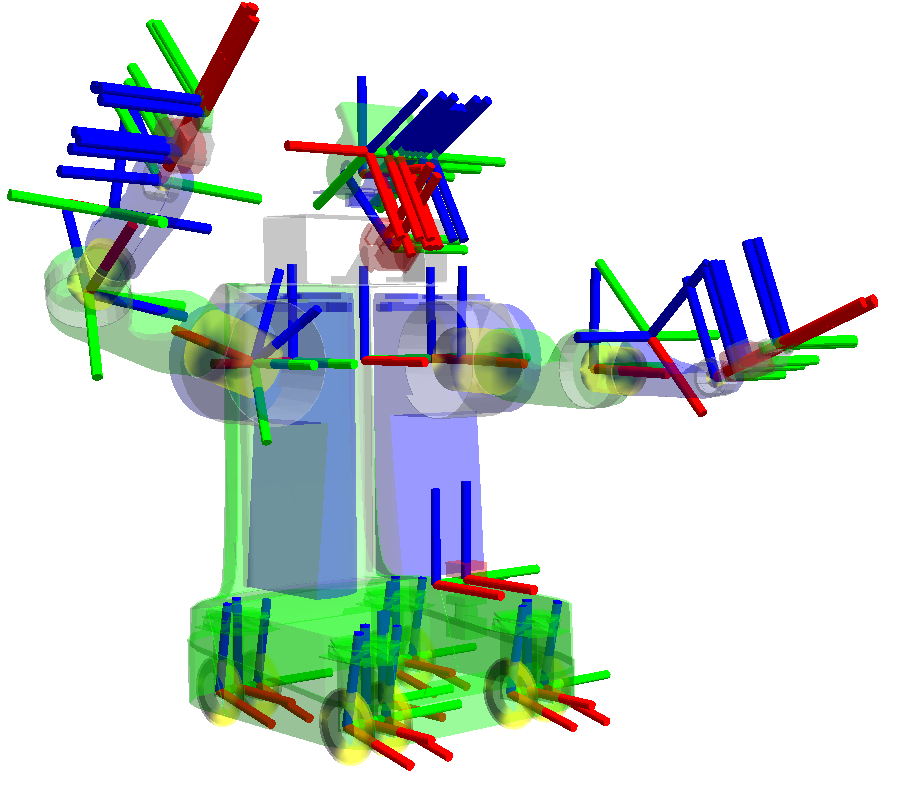
\includegraphics
			[scale=0.35]
			{robot_tf}
		\caption
			[Caption for LOF]{Schematische Darstellung eines Roboters und dessen beweglicher Teile. Die Ausrichtung der jeweiligen Gelenke wird mit einem lokalen Koordinatensystem beschrieben. Die globale Position einzelner Teile kann durch eine Verkettung der relativen Transformation in Richtung der Wurzel des Baumes bestimmt werden.
			Bild aus: \cite{ros_tf_image}}			                                                                                                                                     
		\label{fig:robot_tf}
	\end{figure}

Auch räumliche Daten wie zum Beispiel Punktenwolken aus Laserscannern können relativ zu verschiedenen Koordinatensystemen gesehen werden.
So kann es nützlich sein die Punktwolke relativ zum Koordinatensystem des Scanners oder innerhalb des globalen Koordinatensystems zu betrachten. Um zwischen den Koordinatensystemen zu wechseln wird eine Koordinatensystemtransormation. Diese werden im folgenden Kapitel behandelt.

 
\subsubsection{Transformationen}
\label{section:transformationen}

Eine Koordinatensystemtransformation ist ein Sonderfall einer mathematischen Transformation, die eine Menge $X$ auf sich selbst abbildet:
\begin{myequation}
f: X \rightarrow X
\end{myequation}

Eine Koordinatensystemtransformation beschreibt die Differenz zwischen zwei unterschiedlichen Koordinatensystemen und enthält sowohl die Translationsdifferenz als auch die Rotationsdifferenz.
Zur Berechnung dieser Transformation zwischen zwei beliebigen Koordinatensystem $C_1$ und $C_2$ wird die absolute Translation und Rotation beider Koordinatensysteme zum Ursrungskoordinatensystem, wie zum Beispiel den Urpsrung einer Umgebungskarte, benötigt.
Durch diese Rotations und Translationskomponenten beschreibt sich die absolute Position und Rotation der Koordinatensysteme im Raum aus Sicht des Ursprungskoordinatensystems $C_{MAP}$. Diese absolute Position und Rotation ist die Transformation von den jeweiligen Koordinatensystemen ins Urpsrungskoordinatensystem.

Es existieren diverse Darstellungsweisen für Koodinatensystemtransformationen. Die intuitivste Weise der Darstellung ist die Darstellung als Vektor. In folgendem ist die Transformation vom Koordinatensystem $C_X$ ins Koordinatensystem $C_{MAP}$ dargestellt. Die Variablen $t_i$ bezeichnen dabei die Translationskomponenten und die Variablen $r_i$ die Rotationskomponenten um die jeweiligen Achsen. 

\begin{myequation}
T_{C_X \rightarrow C_{MAP}} = \colvec{t_x\\t_y\\t_z\\r_x\\r_y\\r_z}
\end{myequation}

Neben der Vektordarstellung kann eine Transformation zusätzlich als eine $4x4$ Matrix dargstellt werden.
Diese Darstellungsweise hat den Vorteil, dass die Transformation direkt per Matrixmultiplikation auf Daten wie um homogene Koordinaten erweiterte Punktdaten angewandt werden kann.
Auch die direkt Kombination verschiedener Transformationen ist durch eine Matrixmultiplikation möglich. Hier gilt es zu beachten, dass Matrixmultiplikation nicht kommutativ ist und ein Vertauschen der Reihenfolge bei der Multiplikation zu unterschiedlichen Ergebnissen führen kann.
Bei einer Verkettung von Transformationen durch Multiplikation wird die Matrix zuerst angewandt, welche am Ende der Multiplikation steht.

In dieser Arbeit werden Transformationen zum Beispiel verwendet um zu bestimmen, wie sich ein Roboter zwischen zwei Messungen bewegt hat. Diese Transformationen beschreiben relative Differenzen zwischen Roboterpositionen im Raum. Diese Roboterpositionen werden auch \textbf{Posen} genannt.
Eine Pose ist dabei eine meist absolute Beschreibung der Translation und Rotation eines Roboters zu einem gewissen Zeitpunkt $t$ aus Sicht des Ursprungskoordinatensystems wie zum Beispiel dem Map-Ursprung $C_{MAP}$.


\begin{figure}
		\centering
		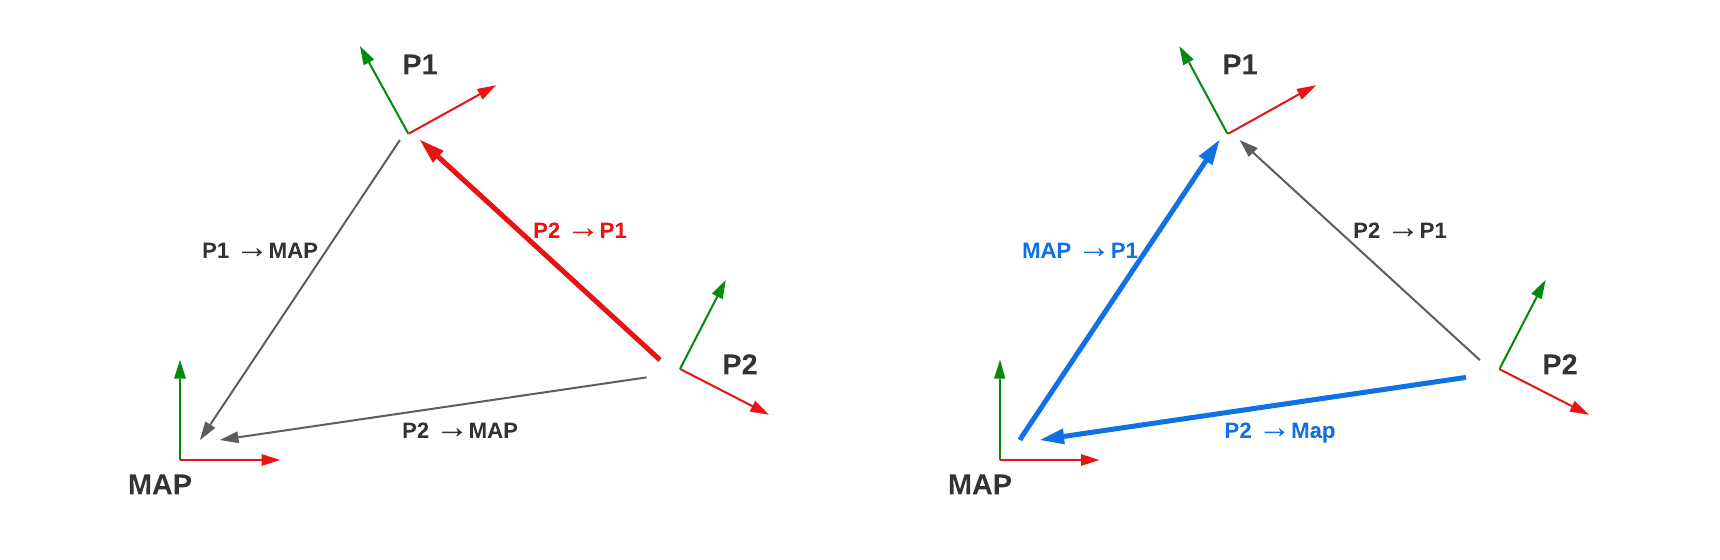
\includegraphics
			[scale=0.25]
			{transformation}
		\caption
			[Caption for LOF]{Schematische Darstellung der bestimmung einer Transformation zwischen zwei Roboter-Posen $P_1$ und $P_2$, hier zur Vereinfachung dargestellt in 2D. Gesucht ist die Transformation $\left( T_{P_2 \rightarrow P_1} \right)$, dargestellt im linken Teil der Abbildung als roter Pfeil. Diese kann implizit bestimmt werden durch eine Verkettung der Transformationen $T_{P_2 \rightarrow MAP}$ und $T_{MAP \rightarrow P1}$, hier dargestellt im rechten Teil der Abbildung in blau. Die Transformation $T_{MAP \rightarrow P1}$ ist dabei nicht explizit gegeben. Sie kann berechnet werden durch eine Inversion der Transformation $T_{P1 \rightarrow MAP}$. Die finale Gleichung zur Berechnung der relativen Transformation ist dargestellt in Gleichung \ref{equation:transformation}.}			                                                                                                                                     
		\label{fig:transformation}
	\end{figure}


Abbildung \ref{fig:transformation} zeigt die Mathematik hinter der Berechnung der Posedifferenz exemplarisch. Es wird deutlich, dass eine gesuchte Transformation aus dem Koordinatensystem von Pose $P_2$ in das Koordinatensystem von Pose $P_1$  $\left( T_{P_2 \rightarrow P_1} \right)$ gegeben ist durch:

\begin{myequation}
\label{equation:transformation}
\left( T_{P_2 \rightarrow P_1} \right) = \left(T_{P_1 \rightarrow MAP} \right)^{-1} * T_{P_2 \rightarrow MAP}
\end{myequation}

Basierend auf den erläuterten mathematischen Grundlagen wird in Kapitel \ref{section:slam} die Grundlagen von SLAM, insbesondere von TSDF basierten SLAM Verfahren, erörtert.
Zuvor werden in nachfolgender Sektion die Eigenschaften und Anwendungsbereiche der TSDF beschrieben.

\section{TSDF}
\label{section:tsdf}

Zur Lösung des \textbf{Simulatneous Localization and Mapping (SLAM)} (siehe Kapitel \ref{section:slam}) Problems in unbekannten Umgebungen wird im Regelfall eine Form der Kartenrepräsentation und die Algorithmik benötigt sich auf Basis der Kartenrepräsentation zu lokalisieren und diese im Anschluss aktualisieren zu können.
Bei vielen Lösungsansätzen wie zum Beispiel einer inkrementellen \textbf{Registrierung (siehe Kapitel \ref{section:slam})} mit dem \textbf{Iterative Closest Point (ICP)} \cite{Besl:1992} oder \textbf{Generalized Iterative Closest Point} \cite{segal2009generalized} Algorithmus werden als Kartenrepräsentation registrierte Punktwolken verwendet.
Punktwolken stellen dabei keine geschlossenen Oberflächenrepräsentationen dar und benötigen viel Speicher im Gegensatz zu einigen geschlossenen Repräsentationen wie aus den Punktwolken generierten Dreiecksnetzen.
Ein großer Nutzen einer solchen Repräsentation ist die vereinfachte Lokalisierung und Navigation auf Basis der Kartenrepräsentation. 

Eine weitere Form der geschlossenen Oberflächenrepräsentation der Umgebung sind \textbf{Signed Distance Functions (SDF)}.
Im Gegensatz zu Dreiecksnetzen sind die SDF implizite, volumetrische Beschreibung der Oberfläche \cite{werner2014truncated}. Sie beschreiben die Oberfläche nicht direkt, sondern den Raum um die Oberfläche herum.
Die \textbf{Signed Distance} ist die orthogonale metrische Distanz eines beliebigen Punktes $p$ zur Oberfläche räumlicher Daten, wie zum Beispiel Punktwolken.
Diese Distanz kann sowohl negativ, als auch positiv sein. Unterschieden wird zwischen dem Innenbereich und Außenbereich.
Abbildung \ref{fig:tsdf} zeigt ein zweidimensionales, schematisches Beispiel für eine diskretisierte TSDF nach Abtasten der Oberfläche einer unbekannten Umgebung durch einen Laserscanner.

\begin{figure}
		\centering
		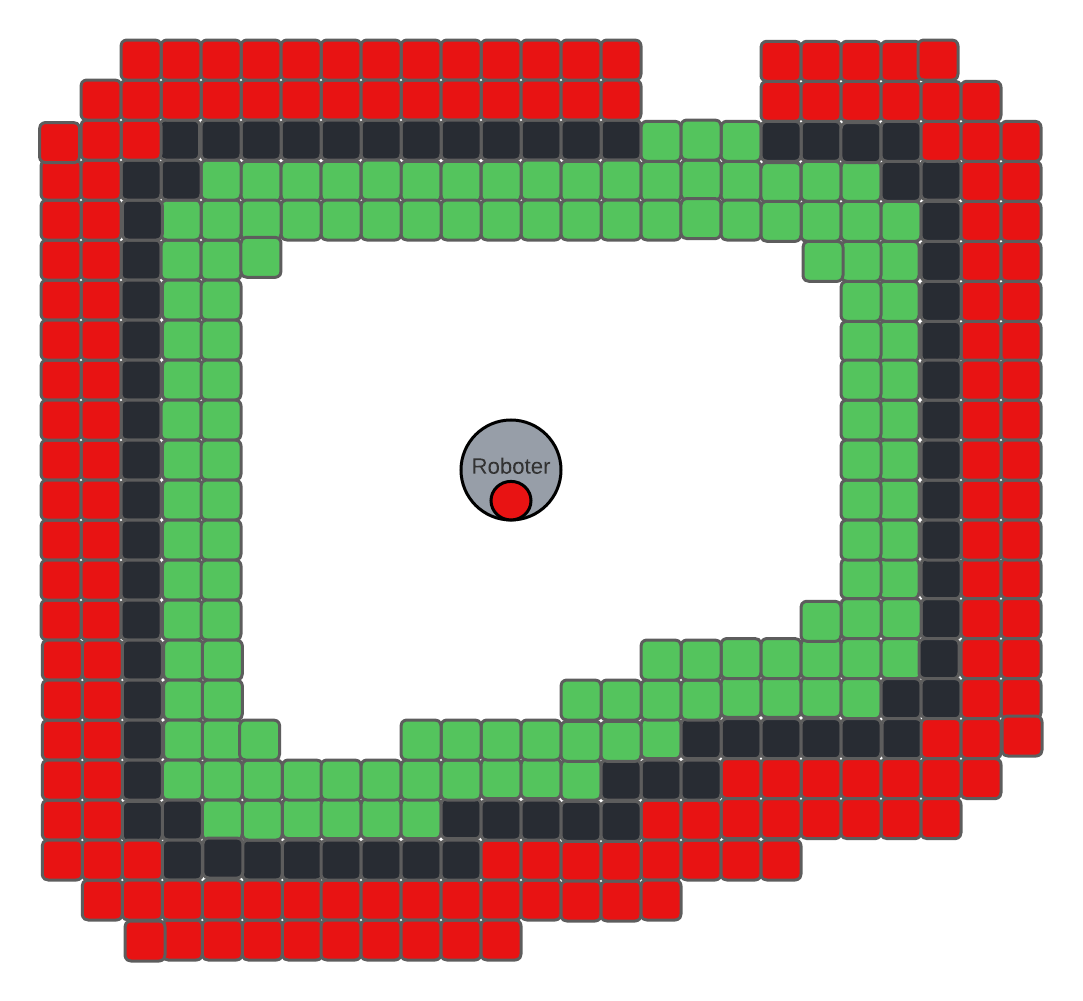
\includegraphics
			[scale=0.3]
			{TSDF}
		\caption
			[Caption for LOF]{Schematische Darstellung einer diskretisierten 2D TSDF Karte. Abgebildet sind nur Voxel mit TSDF-Werten im Intervall $ \left] -\tau, \tau \right[$. In der Mitte der Karte befindet sich ein Roboter mit einem Laserscanner (hier dargestellt in rot). Der Roboter befindet sich zum Beispiel in einem Raum. Der Innenbereich (des Raumes) mit positiven TSDF-Werten ist hier dargestellt in grün, der Außenbereich mit negativen TSDF-Werten in rot. Die Oberfläche, in deren Umgebung die TSDF-Werte nahezu Null sind, ist abgebildet in schwarz.}			                                                                                                                                     
		\label{fig:tsdf}
\end{figure}

Die \textbf{Truncated Signed Distance Funtion (TSDF)} ist eine Unterklasse der SDF. Sie betrachtet die Distanz zur Oberfläche nur bis zu einer maximalen Distanz $tsdf_{max}$, auch $tau \left(\tau)\right)$ gennant\cite{HATSDF}. Alle Werte die weiter von der Oberfäche entfernt oder unbekannt sind, erhalten als Wert $tau$ selbst.
Dies spart Rechenaufwand, da nur die Werte in direkter Nähe zur Oberfläche angepasst werden müssen. In Gebieten, in denen der TSDF-Wert $tau$ entspricht, kann jedoch keine Aussage getroffen werden, wo die nächste Oberfläche ist, oder wie weit sie entfernt ist. Es ist lediglich bekannt, dass die betrachtete Position nicht in direkter Nähe zur Oberfläche befindlich und mindestens $tau$ entfernt ist.
Das Intervall möglicher Werte der TSDF  ist:

\begin{myequation}
I = [-\tau, \tau]:= \lbrace x \in \mathbb{R} \rvert \tau > 0 \rbrace
\end{myequation}

Über SDF und TSDF können kontinuierliche Karten erstellt werden. Da kontinuierliche Karten aber unendlich viel Speicherplatz benötigen, wird der Raum diskretisiert. Die Diskretisierung erfolgt durch eine Aufteilung der Umgebung in \textbf{Voxel} mit definierbarer, fester Seitenlänge $v_{res}$ \cite{whelan2012kintinuous} \cite{HATSDF}. Jeder Voxel enthält einen approximierten (T)SDF-Wert. Diese Form der Darstellung kann auch als pseudo-kontinuierlich angesehen werden, da durch eine Approximation über benachbarte Zellen ein approximierter TSDF-Wert für jeden beliebigen Raumpunkt berechnet werden kann.
Dadurch sind TSDF basierte Karten ideal, um mittels des \textbf{Marching Cubes Algorithmus} \cite{lorensen_marching_1987} eine polygonale Netz-Repräsentation, wie zum Beispiel ein Dreiecksnetz generieren zu können.
Dieses kann zum Beispiel als optische Referenz für die Qualität der Karte verwendet werden.

Eisoldt et al. \cite{HATSDF} basieren ihren SLAM Ansatz auf einer diskreten, inkrementell erweiterten TSDF Karte. Zur Registierung (vergleiche Kapitel \ref{section:slam}) verwenden sie ebenfalls die TSDF-Karte. Punktwolken werden dabei mit einer \textbf{Point-to-TSDF} Strategie an die TSDF Karte registiert \cite{HATSDF}.
In \cite{HATSDF} werden neue Punktdaten nicht an die globale TSDF Karte registriert sondern an eine lokale TSDF Karte fester Größe. Lediglich die lokale Karte befindet sich im Arbeitsspeicher und lädt Daten aus der globalen Karte, die in einer HDF5 Datei repräsentiert wird und auf der Festplatte liegt, nach, sofern eine Repositionierung der Karte notwendig ist.
Dies sorgt dafür, dass \cite{HATSDF} auch für große Umgebungen \textbf{(Large-Scale)} geeignet ist, da der Arbeitsspeicher nicht überläuft.
Abbildung \ref{} zeigt den internen Aufbau einer HDF5 Datei, in der die globale Karte abgespeichert ist.
\improvement{Abbildung einfügen, HDF5 näher beschreiben, Vorteile erklären, referenzieren}
\improvement{TSDF-Update} erklären.

Diese Arbeit beschäftigt sich mit einer möglichen Integration von Schleifenschlüssen in einen auf einer TSDF Karte basierenden Ansatz wie vorgestellt von Eisoldt et al. \cite{HATSDF}. Ziel ist die Korrektur von Fehlern bei der Registrierung und der damit Verbundenen Korrektur der TSDF-Karte. Dies ist in Kapitel \ref{chapter:loop_closure} und \ref{chapter:map_update} beschrieben.

Nachfolgende Sektion behandelt des Thema SLAM und gibt einen groben Überblick über einige SLAM Ansätze. 


\section{SLAM}
\label{section:slam}

Diese Sektion befasst sich mit den Grundlagen von SLAM, stellt heraus welche Varianten von SLAM Verfahren es gibt und wie sich TSDF basierte Verfahren, insbesondere der HATSDF-SLAM Ansatz von Eisoldt et al. \ref{TODO} von diesen unterscheidet.

SLAM ist der Prozess der simultanen Generierung einer Karte einer unbekannten Umgebung und der Lokalisierung innerhalb dieser Karte beziehungsweise Umgebung.
SLAM ist ein \textit{Henne-Ei-Problem}, da auf der einen Seite eine vollständige Karte benötigt um die Pose des Roboters akkurat zu bestimmen, auf der anderen Seite allerdings eine akkurate Posenhistorie benötigt wird um eine gute Karte der Umgebung aufbauen zu können.
Eine grobe Übersicht über existierende SLAM Verfahren liefert der Stand der Forschung in Kapitel \ref{section:sdf}.
Im Folgenden werden einige der genannten Verfahren erneut aufgegriffen und erläutert.
Schlussendlich wird erklärt, welche der SLAM Verfahren für diese Masterarbeit von Interesse sind und wie sie genutzt werden.

Der \textbf{Incremental Closest Points (ICP)} Algorithmus nach Besl und McKay \cite{Besl:1992} ist ein Algorithmus zur \textbf{Registrierung} von Punktwolken.
Als \textbf{Registierung} wird der Prozess der Zusammenführung von Punktwolken bezeichnet, die von unterschiedlichen Orten aus aufgenommen werden. Um Punktwolken möglichst gut zusammenzuführen, wird versucht die aus den Laserscans entstandenen Punktwolken maximal zu überlappen. Dieser Prozess wird auch \textbf{Scan Matching} genannt.
Beim Scan Matching wird zwischen dem \textbf{Model} und dem \textbf{Scan} unterschieden.
Als Scan bezeichnet werden die Daten, die an das Model registiert werden sollen.
Das Ergebnis des Scan Matching ist eine Approximation der Transformation $T_{Scan \rightarrow Model}$ zwischen den Posen von denen aus die Punktwolken aufgenommen wurden.
Damit untersucht werden kann, wie gut diese Approximation ist, liefern ICP und verwandte Algorithmen wie zum Beispiel \textbf{Generalized Incremental Closest Points} \cite{segal2009generalized} ein Maß für die Genauigkeit der Approximation. Dies ist im Fall von ICP und GICP der sogenannte \textbf{Fitness-Score}. Er beschreibt die durchschnittliche quadrierte Distanz zwischen den \textbf{Nearest Neighbors (nächsten Nachbarn)} der Punktwolken nach Anwendung der approximierten Transformation $T_{Scan \rightarrow Model}$ der Scanpunktwolke in das Koordinatensystem der Modelpunktwolke.
Er gibt dementsprechend an, wie groß die durschnittliche quadrierte Distanz eines Punktes aus der Modelpunktwolke zum euklidisch nächsten Punkt der transformierten Scanpunktwolke ist.

Sowohl ICP, als auch GICP sind inkrementelle Algorithmen, dass heißt sie nähern sich inkrementell einem Optimum immer weiter an. Dabei wird die approximiert Transformation jeweils um ein $\delta T$ verändert. Fällt dieses $\delta T$ in einer Iteration unter einen vom Benutzer gewählten Schwellwert, oder wird eine maximale Anzahl an Iterationen erreicht,bricht der Algorithmus ab und gibt die finale Transformation zurück.
Genanntes Optimum ist dabei im Regelfall allerdings kein globales, sondern lediglich ein lokales Optimum aus dem weder ICP noch GICP herauskommen, sobald sie hineingeraten.
Aus diesem Grund gilt es die jeweiligen Ausgaben der Algorithmen zum Beispiel basierend auf dem resultierenden Fitness-Score zu analysieren. 

Beide Algorithmen werden in Kapitel \ref{section:loop_closure_basics} und Kapitel \ref{chapter:loop_closure} in Bezug auf die Identifikation von Loop-Closures evaluiert.

\improvement{Einzelne Verfahren näher beschreiben, erklären welche Bibiloheken verwendet werden}

Varianten (auf die eingegangen wird): 

ICP
Graph-SLAM -> Global Relaxation


 

1. Grundlagen von SLAM beschreiben
-> Varianten des SLAM
-> Bezug zu HATSDF-SLAM
2. Vorraussetzungen (Repräsentationen für Posen (Pfad) und Umgebung)
3. Überleitungen in weitere Sektionen machen
	-> Loop Closure als mögliche Verbesserung des SLAM
	-> TSDF als Kartenrepräsentation
		-> auf Vorteile von TSDF eingehen (z.B. einfache Integration in Marching Cubes Algorithmus)



\section{Loop Closure}
\label{section:loop_closure_basics}

Warum wird Loop Closure benötigt?
Welchen Mehrwert gibt es?
Wie wäre ein grundlegendes vorgehen?
verweisen auf Loop-Closure Kapitel